% !TeX root = text.tex
\documentclass{template/socthesis}

\usepackage{subcaption}
\usepackage{amsmath}
\usepackage{enumitem}

% my~own code
\usepackage{xkvltxp}

\usepackage[skip=10pt plus1pt, indent=0pt]{parskip}
\usepackage[polutonikogreek,czech]{babel}
\usepackage{float}
\usepackage{geometry}
\usepackage{gensymb}
\usepackage{amssymb}
\usepackage[T1]{fontenc}
\usepackage[utf8]{inputenc}
\usepackage{minted}
\setmintedinline{breaklines}

\usepackage{subcaption}
\usepackage{caption}

\usepackage[pages=some]{background}
\backgroundsetup{
  scale=1,
  angle=0,
  opacity=1,
  color=black,
  contents={%
    \includegraphics[width=\paperwidth,height=\paperheight]{img/pcb-schem-full.jpg}
  }
}

\usepackage[author=,status=draft]{fixme}
\makeatletter
\renewcommand*\FXLayoutInline[3]{%
  {\@fxuseface{inline}\ignorespaces[#2]}}
\makeatother

\usepackage{caption}
\DeclareCaptionType{equ}[Rovnice][Seznam rovnic]
%\captionsetup[equ]{labelformat=empty}

\widowpenalty=5000
\clubpenalty=5000
\brokenpenalty=5000

%%%%%% podbarvení bloků kódu / vygenerovaných ai
\usepackage{xcolor}
\usepackage{listings}
\usepackage{tcolorbox}

\tcbuselibrary{breakable}

\definecolor{aiblue}{rgb}{127,127,255}
\definecolor{aibackground}{rgb}{100,100,100}

\lstdefinestyle{aistyle}{
    backgroundcolor=\color{aibackground},   
    commentstyle=\color{aiblue},
    keywordstyle=\color{aiblue},
    numberstyle=\tiny\color{aiblue},
    stringstyle=\color{aiblue},
    basicstyle=\ttfamily\footnotesize,
    breakatwhitespace=false,         
    breaklines=true,                 
    captionpos=b,                    
    keepspaces=true,                 
    numbers=left,                    
    numbersep=5pt,                  
    showspaces=false,                
    showstringspaces=false,
    showtabs=false,                  
    tabsize=2
}

% https://tex.stackexchange.com/questions/24528/having-problems-with-listings-and-utf-8-can-it-be-fixed
\lstset{style=aistyle,
inputencoding=utf8,
extendedchars=true,
literate=%
{á}{{\'a}}1
{č}{{\v{c}}}1
{ď}{{\v{d}}}1
{é}{{\'e}}1
{ě}{{\v{e}}}1
{í}{{\'{\i}}}1
{ň}{{\v{n}}}1
{ó}{{\'o}}1
{ř}{{\v{r}}}1
{š}{{\v{s}}}1
{ť}{{\v{t}}}1
{ú}{{\'u}}1
{ů}{{\r{u}}}1
{ý}{{\'y}}1
{ž}{{\v{z}}}1
{Á}{{\'A}}1
{Č}{{\v{C}}}1
{Ď}{{\v{D}}}1
{É}{{\'E}}1
{Ě}{{\v{E}}}1
{Í}{{\'I}}1
{Ň}{{\v{N}}}1
{Ó}{{\'O}}1
{Ř}{{\v{R}}}1
{Š}{{\v{S}}}1
{Ť}{{\v{T}}}1
{Ú}{{\'U}}1
{Ů}{{\r{U}}}1
{Ý}{{\'Y}}1
{Ž}{{\v{Z}}}1
}

\DeclareUnicodeCharacter{2212}{\textminus}% requires a~unicode capable editor

\addbibresource{text.bib}

\titlecz{RGB Laserový projektor}
\titleen{RGB Laser projector}
\author{Šimon Hrouda}
\field{10}
\school{Gymnázium Brno-Řečkovice, p.~o., Terezy Novákové 2, 621 00 Brno}
\mentor{Tomáš Rohlínek a~Mgr.~Kateřina Vídenková}
\mentorstatement{Tomáše Rohlínka a~Mgr.~Kateřiny vídenkové}


% Změňte, pokud se~liší
%\region{Jihomoravský}
\placefooter{Brno 2024}

\begin{document}
% \newcommand{\bard-gen}[3]{text vygenerován ai~#1}
\newcommand{\bardgen}[3]{following text generated by~ai~(google bard) on~#1\\%
  \begin{tcolorbox}[breakable, colback=blue!20]
    #2
  \end{tcolorbox}
  \begin{tcolorbox}[breakable, colback=blue!10, colframe=white]
    #3
  \end{tcolorbox}
}


\maketitle

\makecopyrightstatement{V~Brně}

\makethanks{Děkuji svému externímu konzultantovi Tomáši Rohlínkovi a~své interní konzultantce Mgr. Kateřině Vídenkové za~obětavou pomoc, podnětné připomínky a~nekonečnou trpělivost, kterou mi~během práce poskytovali.}

\pagestyle{empty}

\section*{Anotace}


\subsection*{Klíčová slova}


\vspace{20mm}

\section*{Annotation}


\subsection*{Keywords}


\newpage
\pagestyle{plain}

\tableofcontents % vysází obsah

%%% Začátek práce
\setcounter{figure}{0}
\setcounter{table}{0}

\newpage

definice pojmů a~zkratek
\begin{center}
  \begin{tabular}{c c c}
    SPI  & Serial Peripheral Interface     & sériové periferní rozhraní            \\
    DPS & & deska plošných spojů \\
  \end{tabular}
\end{center}

% !TeX root = text.tex
\chapter*{Úvod}
\addcontentsline{toc}{chapter}{Úvod} % přidá položku úvod do~obsahu

% \fxnote{?když jsem se~zajímal o~technologii laserových projektoru a~efektu na~diskotekach, zarazilo mě, že jsem nenašel žádnou open source platformu, kterou bych mohl použít a~případně upravovat, kdybych chtěl techcnologii využít, tak jsem se~rozhodl takovou platformu vytvorit}

Laser scanning, technologie rychle se~pohybujícího laserového paprsku, je~využívána v~mnoha oblastech od~laserového promítání, efektů na~diskotékách a~průhledových displejů~(Průhledový displej -- anglicky Head-Up Display (HUD)) v~letadlech, autech či brýlích pro rozšířenou realitu~\cite{laser-huds} přes čtení čárových kódů~\cite{history-of-barcode-scanning} a~3d tisk~\cite{Photo-curing-3D-printing} po~skenování 3D modelů~\cite{3d-model-scan} i~Zemského povrchu~\cite{heightmaps}.

Bohužel ale neexistují žádné uživatelsky přívětivé open-source platformy, kde by~se~s~touto technologií mohli seznámit zájemci o~její rozvíjení.

\subsection*{Cíle}
\addcontentsline{toc}{subsection}{Cíle} % přidá položku úvod do~obsahu
V této práci jsem se~proto rozhodl pro tuto technologii vytvořit vlastní laserový projektor a~naprogramovat pro něj jednoduché uživatelské prostředí.
Toto uživatelské prostředí by~mělo sloužit jako začáteční bod, který zaujme mladé zájemce a~umožní jim si~technologii vyzkoušet.
V případě, že techologie zaujme, mělo by~pro zájemce být jednoduché program pozměnit nebo si~jinak .
% \fxnote{QUESTION\_INTERNAL: jak sepsat cíle? tenhle odstavec tam hezky sedí, ale zvyklejsí jsou asi odrazky, ne?}


% \input{100-uvod-teor.tex}

\chapter{Laser scanning~\cite{scanning-handbook}}
Všechny obrázky v této kapitole pocházejí ze~zdroje~\cite{scanning-handbook}, pokud není uvedeno jinak.

Jako Laser scanning se~označuje technologie využívající rychle pohybující laserový paprsek, tento pohyb je~často zprostředkovaný pohyblivými zrcátky.

Dle stylu pohybu zrcátek se~technologie dají rozdělit na, polygonové skenery, galvanometrové a~MEMS skenery.

\section{Hranolové skenery}
Hranolové skenery se~vyznačují rotujícím hranolem se~zrcadlivými stranami (dále \uv{zrcátky}). Při rotaci hranolu se~mění úhel dopadu laserového paprsku na~zrcátko, a~díky tomu se~mění směr odraženého paprsku, viz. obrázek \ref{fig:polygon-scanner}. \fxnote{adiky carka?}

\begin{figure}[H]
  \centering
  \includegraphics[width=0.5\textwidth]{img/polygon-scanner.jpg}
  \caption{\label{fig:polygon-scanner} mechanika polygonových skenerů}
\end{figure}

% \begin{figure}[!htb]
%   \centering
%   \includegraphics[width=0.5\textwidth]{img/polygon-prismatic-mirror.jpg}
%   \caption{\label{fig:polygon-prismatic-mirror} hranolové zrcátko polygonového skeneru}
% \end{figure}

% \begin{figure}[!htb]
%   \centering
%   \includegraphics[width=0.5\textwidth]{img/polygon-pyramidal-mirror.jpg}
%   \caption{\label{fig:polygon-pyramidal-mirror} pyramidové zrcátko polygonového skeneru}
% \end{figure}
%

S jedním hranolem by~hranolové skenery byly schopny směřovat paprsek pouze v~jedné rovině - při projekci by~bylo možné vykreslit maximálně čáru. Tuto limitaci lze kompenzovat přidáním melého rozdílu ve~směřování každé strany hranolu, viz. obrázek \ref{fig:polygon-angular-variation}. S~touto úpravou každá strana hranolu "vykreslí" jednu, svoji, přímku lehce posunutou vůči přímkách ostatních stran. Hranol s~n-úhelníkovou podstavou je~schopen vykreslit n~přímek.
Další možností je~kombinovat původní pravidelný hranol s~galvanometrem (popsáno níže), kdy galvanometr nastaví jednu souřadnici paprsku a~hranol na~této souřadnici vykreslí přímku.

Tento typ skeneru se~využívá hlavně pro senzory skenující na~přímce (např. skenery čárových kódů~\cite{history-of-barcode-scanning}), nebo při rastrovém procházení plochy (například 3D skenování, nebo promítání ploch, viz. Obrázek \ref{fig:harddrive-projector-youtube}).

\begin{figure}[!htb]
  \centering
  \includegraphics[width=0.8\textwidth]{img/polygon-angular-variation.jpg}
  \caption{\label{fig:polygon-angular-variation} úhlová rozdílnost zrcátek polygonového skeneru a~paprsky od~nich odražené}
\end{figure}


\begin{figure}[!htb]
  \centering
  \includegraphics[width=0.5\textwidth]{img/harddrive-projection.jpg}
  \caption{\label{fig:harddrive-projection} příklad projekce laserového projektoru s~polygonovým skenerem; zdroj~\cite{harddrive-projector-youtube}}
\end{figure}

\section{Galvanometrové skenery}
V galvanometrových skenerech paprsek odráží zrcátka/o připevněná/o na~páru galvanometrů.

\subsection{Galvanometr}
Slovem galvanometr se~označuje přístroj úrčený k~detekci nebo měření velice malého elektrického proudu~\cite{galvo-definition}. Galvanometry při měření využívají interakce magnetického pole trvalého magnetu a~cívky protéké proudem. Tato interakce vychýlí ručičku ukazující na~stupnici, nebo zrcátko odrážející paprsek, který dopadá na~stupnici.~\cite{wiki-galvo}

Galvanometry se~dají rozdělit na~galvanometry bez zpětné vazby (open-loop) a~se zpětnou vazbou. K~těm bývají připojeny ovládací obvody, které z~galvanometrů získávají informace o~jejich pohybu a~podle nich regulují signál posílaný do~galvanometrů.~\cite{wiki-galvo}

Dále se dělí dle pohyblivé součástky. V galvanometru je buď trvalý magnet pevně ukotven a cívka pohyblivá (moving coil), nebo naopak (moving magnet). % https://prirucka.ujc.cas.cz/?id=151#nadpis3

Dnes se~v~kontextu laserových skenerů prakticky vždy používají galvanometry s~pohyblivým magnetem a se~zpětnou vazbou. Ta je zajištěna čtením z variabilního kondenzátoru umístěného v galvanometru.

\begin{figure}[!htb]
  \centering
  \includegraphics[width=1\textwidth]{img/galvanometer-detail.jpg}
  \caption{\label{fig:galvanometer-detail} zapojení a vnitřní konstrukce galvanometrů}
\end{figure}

\subsection{Konstrukce galvanometrových skenerů\label{sec:galvo-scanner-construction}}
Jeden galvanometrový skener vždy ovládá jednu osu pohybu paprsku, buď X~nebo Y.

Narozdíl od~hranolových skenerů je~s galvanometrovým skenerem možné zastavit obě osy pohybu - vykreslovat na~sebe kolmé čáry.

\begin{figure}[!htb]
  \centering
  \includegraphics[width=1\textwidth]{img/scanner-constructions.jpg}
  \caption{\label{fig:scanner-constructions} různé konstrukce galvanometrových skenerů}
\end{figure}

\section{Má volba skeneru}
\fxnote{sekce mozna patri do~prakticke}
ja vyuzivam galva, protoze se~s nima da~nejlip pohrat, jsou nejuniverzalnejsi a~tim padem nejvic zaujmou - cil

\chapter{Laserová projekce}
Laserová projekce spadá mezi laser scanning technologie. Často je~využívána v~zábavním průmyslu, hlavně k~vytváření laser shows a~vektorových projekcí. U~laser shows diváci sledují vzory, které vytváří samotný paprsek ve~vzduchu. U~projekcí diváci sledují obrazce vykreslené paprskem dopadajícím na~promítací plátno.~\cite{laser-projection}

Tyto efekty nejsou populární pouze v~klubech, nýbrž i~na~koncertech nebo živých představeních. Je-li laser dostatečně silný, je~možné promítat na~obrovské plochy, jako například hráze, vodní plochy, nebo dokonce hory.~\cite{laser-projection}

\section{Využití laserové projekce v~průhledových displejích~(HUD)}
Laserová projekce se~také využívá v~průhledových displejích. Příklady HUD~jsou vidět na~obrázcích~\ref{fig:hud} a~\ref{fig:hudd}.


\begin{figure}[h]
  \centering
  \begin{minipage}{0.45\textwidth}
    \centering
    \includegraphics[width=0.9\textwidth]{img/hud.jpg}
    \caption{\label{fig:hud} HUD~v letadle Boeing 737-800~\cite{dev-of-laser-huds-in-driving}}
  \end{minipage}\hfill
  \begin{minipage}{0.45\textwidth}
    \centering
  \includegraphics[width=0.9\textwidth]{img/hudd.jpg}
  \caption{\label{fig:hudd} HUD~ve stíhacím letounu F16~\cite{dev-of-laser-huds-in-driving}}
  \end{minipage}
\end{figure}

% \begin{figure}[h]
%   \centering
%   \begin{minipage}{0.45\textwidth}
%     \centering
%   \includegraphics[width=0.9\textwidth]{img/huddd.jpg}
%   \caption{\label{fig:huddd} HUD~v automobilu BMW~5-series~\cite{dev-of-laser-huds-in-driving}}
% \end{minipage}\hfill
% \begin{minipage}{0.45\textwidth}
%   \centering
%   \includegraphics[width=0.9\textwidth]{img/hudddd.jpg}
%   \caption{\label{fig:hudddd} HUD~v automobilu Peugeot 5008~\cite{dev-of-laser-huds-in-driving}}
% \end{minipage}
% \end{figure}

V~tomto odvětví zatím převládají jiné technologie. Technologie průhledových displejů se~dají rozdělit následovně:
\begin{itemize}
  \item Technologie vyzařujících displejů,~např. cathode ray~tube~(CRT), organic light-emitting diode~(OLED) nebo vacuum fluorescent display (VFD).
  \item Technologie podsvícených displejů,~např. liquid crystal display (LCD).
  \item Technologie laserových displejů,~např. liquid crystal on~silicon (LCoS) nebo laser scanning displeje založené na~pohybu mikrozrcadel.~\cite{dev-of-laser-huds-in-driving}
\end{itemize}

V prvních průhledových displejích bylo využito CRT. Ale~kvůli své neskladnosti, vysoké spotřebě elektřiny a~škodlivé radiaci, byla nahrazena technologií LCD. Dnes se~v~průhledových displejích letadel využívají LCD. V~automobilech se~využívají LCD~a~VFD.
Bohužel VFD~jsou limitovány množstvím informací, které mohou zobrazit. LCD~průhledové displeje jsou limitovány svým maximálním jasem.
S novou technologií OLED sice je~možné vytvořit tenký a~průhledný displej dosahující vyšího jasu než LCD~HUD.
I tento displej bohužel oproti vnějšímu světu má stále relativně nízký jas, také má vysokou cenu a~krátkou životnost.
Oproti vyzařujícím a~podsvíceným displejům jsou laserové displeje nadřazené.~\cite{dev-of-laser-huds-in-driving}

\section{Princip laserové projekce}\label{sec:projection-princip}
Když se~laserový paprsek pohybuje dostatečně rychle, lidské oko~ho~vnímá jako spojitou linku světla -- tomuto jevu se~říká \It{persistance of~vision} nebo \It{persistance of~impression}~\cite{persistance-of-vision}.
Čím rychleji se~paprsek pohybuje, tím méně intenzivní připadá oku~zmíněná linka. Bod~je~možné vykreslit, jestliže paprsek zůstane na~jednom místě bez~pohybu po~úrčitou dobu.~\cite{laser-projection}

Vykreslení čáry je~základní a~nejjednoduší operací, jakou laserový projektor může vykonat. Například k~vykreslení úsečky z~bodu A~do~bodu B~projektor nasměřuje laserový paprsek na~bod~A, zapne laser a~pohybuje paprskem k~bodu B.~\cite{laser-projection}

K vykreslení složitějších obrázků jsou potřeba tzv. blank\ lines, kdy~projektor otáčí zrcátky stejně, jako kdyby vykresloval přímku, ale~laser nesvítí. Blank lines spojují každé dvě vykreslené linky, které na~sebe přímo nenavazují.~\cite{laser-projection}

Nestihne-li projektor vykreslovat obraz dostatečně rychle, výsledná projekce nebude stabilní. Lidské oko~vždy uvidí pouze části obrazu v~časové návaznosti. Tomuto jevu se~říká \uv{flickering}.~\cite{laser-projection}

Příklad obrazu vykresleného laserovým projektorem je vidět na obrázku~\ref{fig:gyrec}. Na tomto obrázku foto aparát zachytil i částečný \uv{flickering}, pro lidské oko ovšem nebyl viditelný.

\begin{figure}[htb]
  \centering
  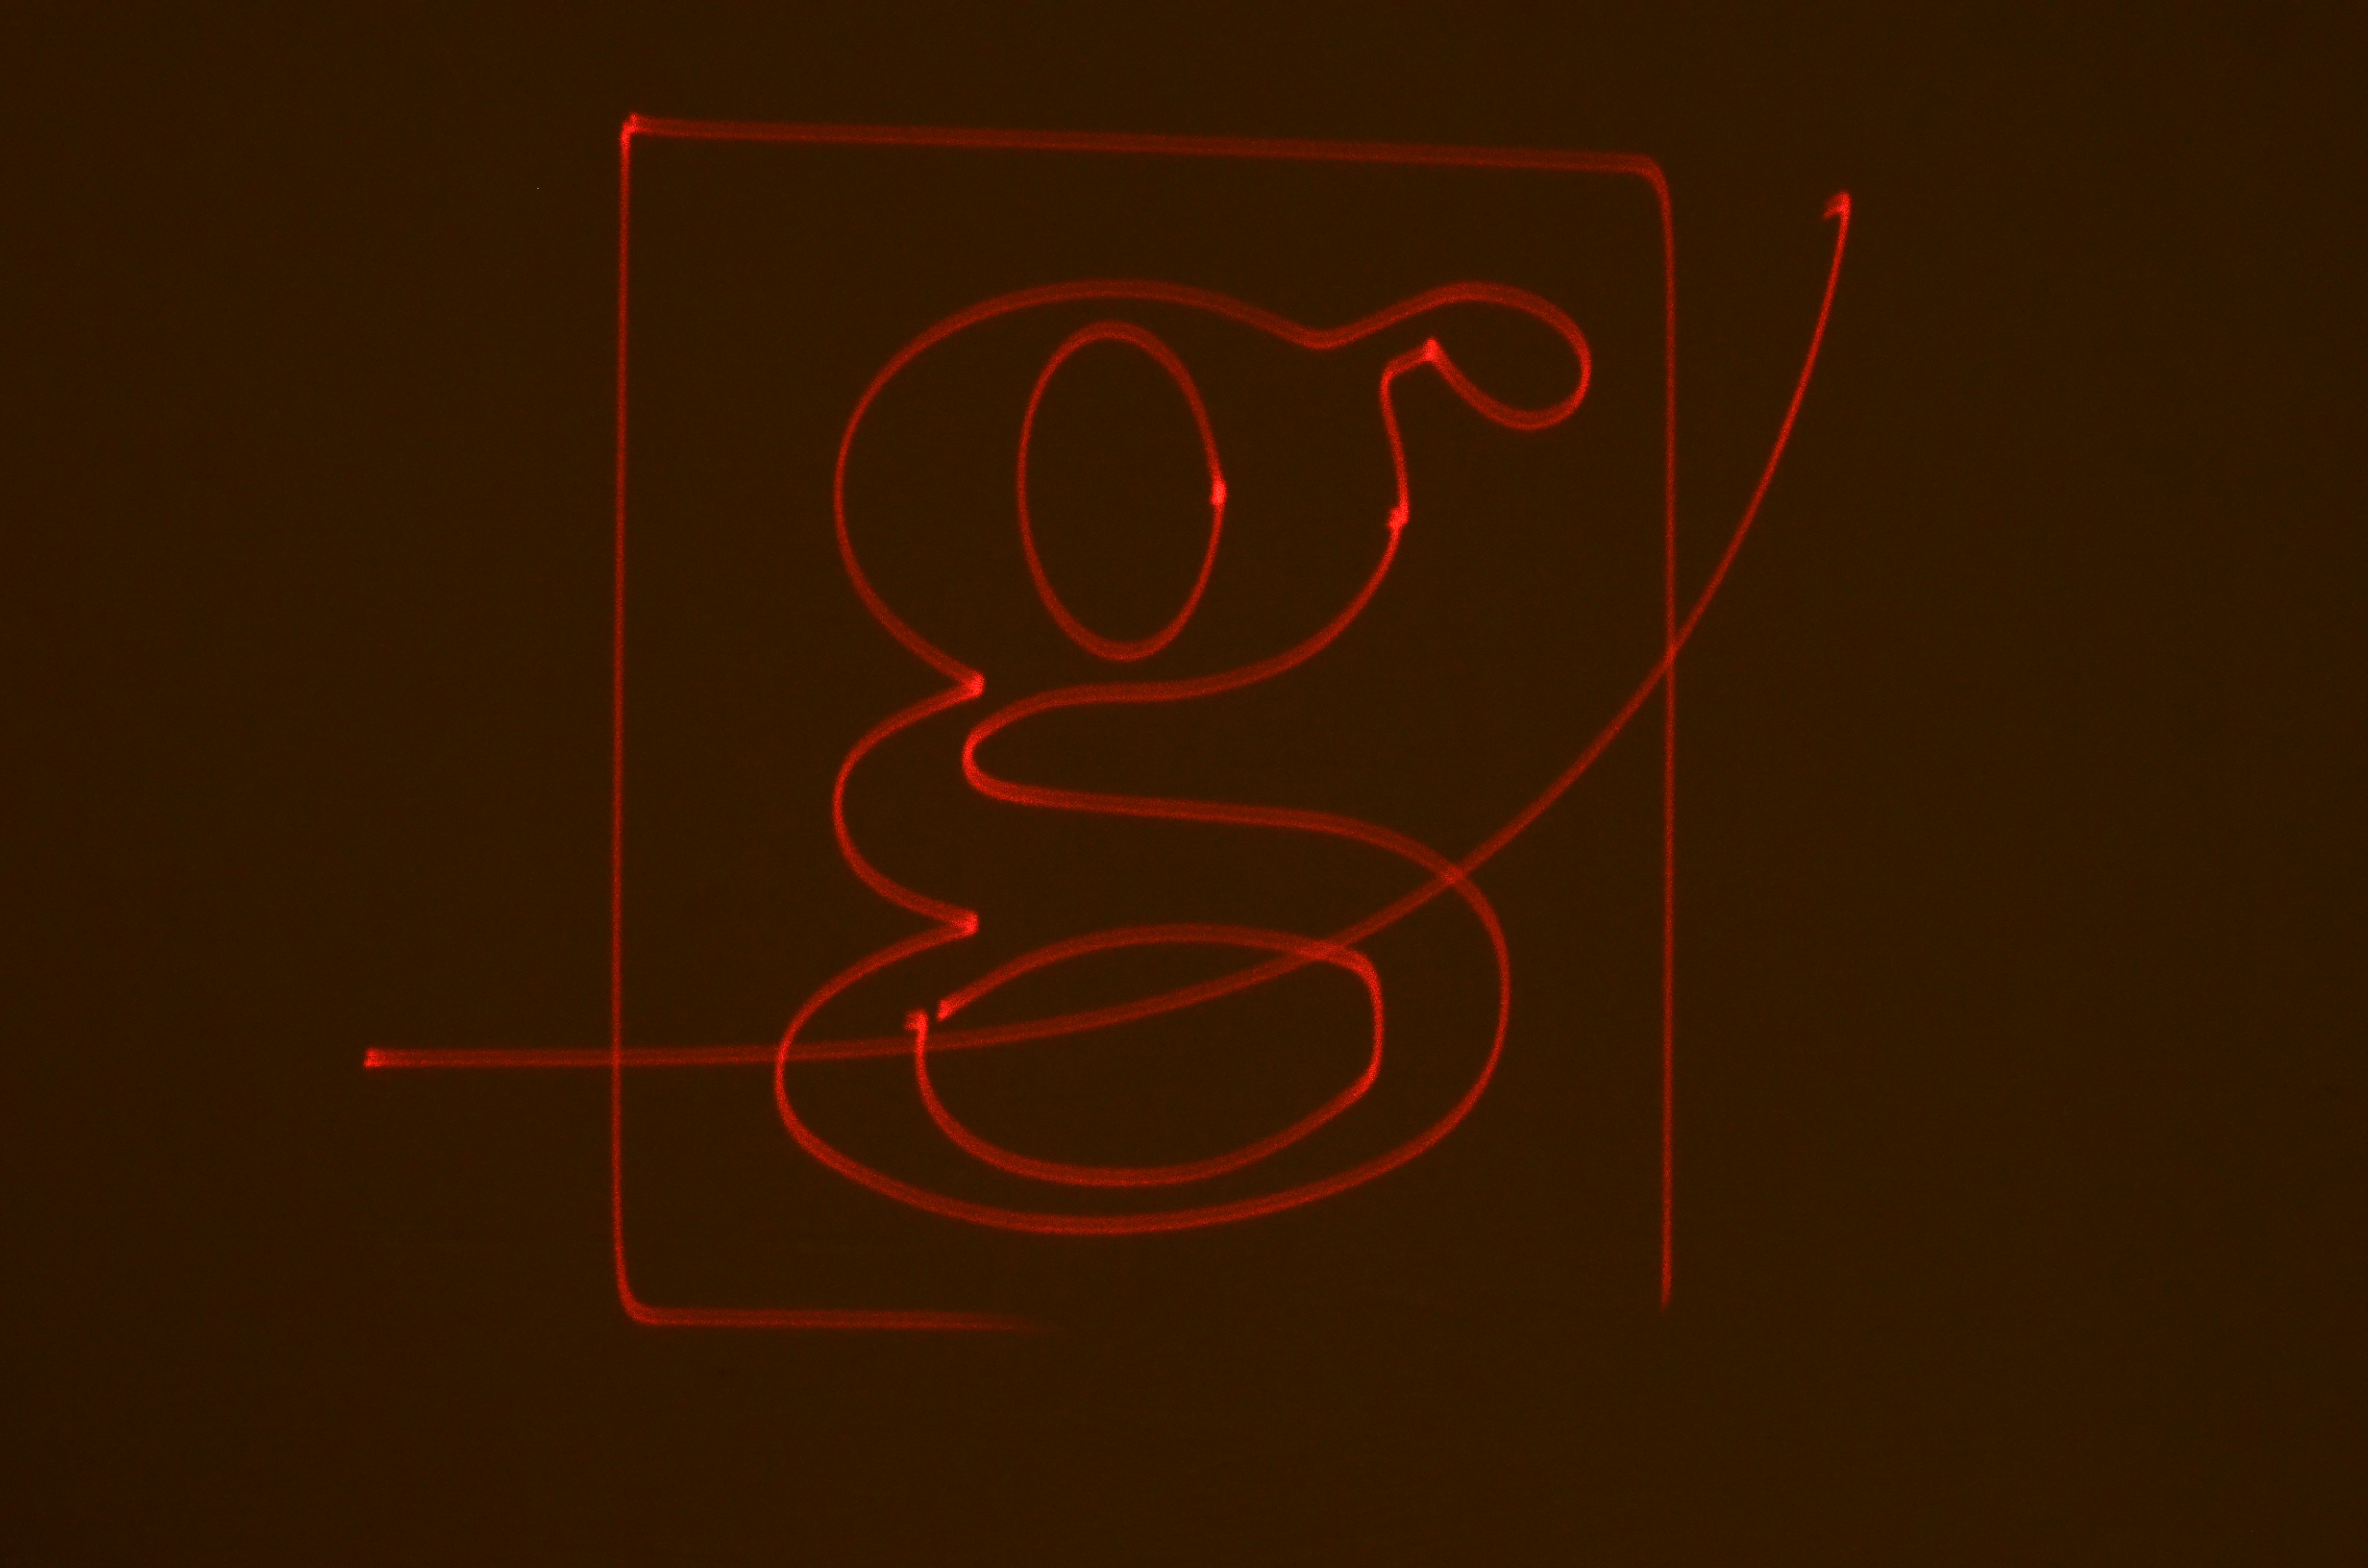
\includegraphics[width=1\textwidth]{img/gyrec.JPG}
  \caption{\label{fig:gyrec} Ukázka projekce; doba závěrky fotoaparátu 1/30~s}
\end{figure}

\chapter{Laser safety}
\fxnote{citovat z \url{https://dspace.vut.cz/server/api/core/bitstreams/a55c1118-9166-4449-806a-c2a73bfeff66/content}}

3.3 Laserová bezpečnost [7,8]
Při práci s lasery vzniká možnost ohrožení zdraví laserovým zářením. Podle nařízení vlády
č. 1/2008 Sb. O ochraně zdraví před neionizujícím zářením, ve znění pozdějších předpisů se
optickým zářením se pro účely tohoto nařízení rozumí záření z umělých zdrojů odpovídající
vlnovým délkám od 100 nm do 1 mm, jehož spektrum se dělí na:
• ultrafialové (100 nm až 400 nm)
• viditelné záření (380 nm až 780 nm)
• infračervené (780 nm až 1 mm)
Laserem se rozumí jakékoliv zařízení, které je určeno k vytváření nebo zesilování
elektromagnetického záření primárně procesem kontrolované stimulované emise. Laserová
záření jsou elektromagnetické vlny stejné fyzikální podstaty jako vlny vznikající v přírodě,
ovšem jejich intenzita a rovnoběžnost svazku je podstatně vyšší. V případě vystavení člověka
působení laserového záření vzniká nebezpečí újmy na zdraví, postihující nejvíce oči a kůži.
Ve většině případů se nedá před poškozením oka ochránit odkloněním hlavy nebo
zavřením očních víček, jelikož takováto reakce je příliš pomalá. Pro ochranu zdraví jsou tudíž
19
stanovena pravidla, která zaručují, že k poškození zdraví nedojde. Maximální přípustná dávka
ozáření (MPE) je hodnota laserového záření, kdy při vystavení lidské pokožky nebo oka
nedojde k okamžitému nebo pozdějšímu poranění. Hodnota MPE je závislá na vlnové délce,
době ozáření, typu ozařované tkáně a při ozáření oka na velikosti obrazu na sítnici.
V Tabulka 1 jsou upraveny nejvyšší přípustné hodnoty expozice pro přímý pohled do
laserového svazku nebo přímý pohled do zrcadlově odraženého svazku.
Tabulka 1 Nejvyšší přípustná hodnota expozice při přímém působení laserového záření na rohovku oka
(přímý pohled do svazku) [7]
V Tabulka 2 jsou upraveny nejvyšší přípustné hodnoty ozáření rohovky oka při sledování
plošného laserového zdroje nebo laserového svazku po difúzním odrazu.
20
Tabulka 2 Nejvyšší přípustné hodnoty ozáření rohovky oka při pozorování plošného laserového zdroje
nebo laserového svazku po difúzním odrazu [7]
V Tabulka 3 jsou zobrazeny hodnoty nejvyššího přípustného ozáření při expozici
laserového záření na kůži.
Tabulka 3 Nejvyšší přípustné ozáření při expozici laserového záření na kůži [7]
Tabulka 4 Hodnoty konstant pro tabulky výše [7]
21
Korekční faktory použité v tabulkách 1 – 3 jsou vyjádřeny v Tabulka 4.
3.4 Třídy laserů
• 1 – zařízení třídy 1 jsou bezpečná včetně dlouhodobého pozorování světelného
svazku nebo jeho sledování pomocí čoček či dalekohledů. To této kategorie spadají
i vysokovýkonné lasery, které jsou zcela zakrytovány a neumožní průnik paprsku
do okolí, při případném otevření se celé zařízení vypne.
• 1M – zařízení spadající do třídy 1M jsou bezpečná i při dlouhodobém sledování
světelného svazku, nejsou ovšem bezpečná při sledování pomocí optických
pomůcek (čočky, dalekohledy).
• 2 – Jedná se lasery v rozsahu vlnových délek 400 – 700 nm. Přímý dlouhodobý
pohled do světelného svazku může způsobit poškození zraku. Reakční doba lidí při
oslnění (zavření víček, odvrácení hlavy) se pohybuje okolo 0,25s. Pokud člověk při
oslnění do této doby zareaguje, neměl by mít trvale poškozený zrak, může ovšem
dojít ke krátkodobým poruchám vidění, které v pracovních provozech významně
ovlivňují bezpečnost práce.
• 2M – stejné jako třída 2 s tím, že při použití optických pomůcek není garantováno
po vystavení lidského oka záření po dobu do 0,25s, že nedojde k nevratnému
poškození zraku.
• 3R - vyzařované záření může při přímém sledování svazku překročit maximální
přípustnou dávku ozáření, nebezpečí poškození zraku je ovšem relativně nízké,
jelikož limity třídy 3R jsou pouze pětinásobkem třídy 2. Zařízení s laserem třídy
3R by měla být používána pouze tam, kde je pohled do svazku nepravděpodobný.
• 3B – při pohledu do světelného svazku je vážné riziko trvalého poškození zraku,
včetně náhodných a krátkodobých ozáření. Záření z difuzního odrazu jsou běžně
bezpečná. Může dojít k malým poraněním pokožky, laser může být též příčinnou
vzniku požáru.
• 4 – Pohled do laseru spadajícího do třídy 4 je značně nebezpečný, ozáření pokožky
představuje taktéž velké nebezpečí. Nebezpečí mohou představovat i odražené a
rozptýlené paprsky. Laser představuje i riziko vzniku požáru.
Podle [7] je limit pro třídu 3A při působení záření na lidské oko po dobu nad 0,25s 5mW a
25W/m2, limity pro třídu 3B je 0,5W v rozsahu vlnových délek 400 – 700nm.
22
Lasery použité v práci (červený 650nm, 100mW – zelený 532nm, 100mW – modrý 450
nm, 150mW) jsou tedy třídy 3B a přímý pohled do světelného svazku je nebezpečný, světlo z
obrazců vykreslovaných na stěnu a dopadající na sítnici oka vlivem difuzního odrazu není pro
zrak hrozbou.

spi
nodejs
ZeroMQ
3d tisk


% \input{.tex}


% \input{200-uvod-prak.tex}

% !TeX root = text.tex
\chapter{hardware}

\section{Raspberry Pi}
\fxnote{TODO: rpi specs}

\section{Set galvanometrů se~zrcátky} \label{sec:my-galvos}
\subsection{Výběr skeneru}
Pro tuto práci byl vybrán galvanometrový skener, protože je~nejdostupnější a~protože potenciálním uživatelům nejlépe představí technologii.

Oproti hranolovým skenerům jim tožiž dává více možností, jak s paprskem pohybovat.
Můžou se~rozhodnout, že jej využijí jako hranolový skener, pokud nahrají soubor procházející promítací plochu po~řádcích.

Oproti dalším typům skenerů je~názornější, ostatní typy skenerů jsou totiž příliš malé a~není na~nich vidět princip funkce nebo je~jejich fungování nadmíru abstraktní a~těžko pochopitelné.

\subsection{Zapojení galvanometrového setu}
Samotné galvanometry jsou zapojeny do~řídící desky, která s nimi byla zakoupena, ta je vidět na obrázku~\ref{fig:hw_galvoboard}.

Řídící deska požaduje symetrický zdroj napětí 15~V, tzn. $+15$~V a~$-15$~V a~samozřejmě připojení k zemi. Také přijímá dva bipolární diferenciální analogové signály s~rozsahem diferenciálního napětí $-10$~V až $+10$~V. Každý signál udává vychýlení jednoho ze~dvou galvanometrů, což obvykle znamená výslednou pozici laserového paprsku v~osách X~a~Y.

\begin{figure}[htb]
  \centering
  \includegraphics[width=1\textwidth]{img/hw_galvoboard.jpg}
  \caption{\label{fig:hw_galvoboard} Řídící deska galvanometrů s vyznačenými konektory a hřejícími čipy}
\end{figure}

\subsection{bipolární diferenciální analogový signál~\cite{ilda-signal-spec}}
Diferenciální signál je~signál přenášený dvěma vodiči, každý z~nich přenáší stejný signál, jen s~opačnou polaritou. Kontakt označený $(+)$ je~považován za~nosič základního signálu, zatímco kontakt označený $(-)$ je~považován za~nosič invertovaného signálu. Výsledné diferenciální napětí je~napětí na~základním nosiči vůči napětí na~obráceném nosiči, tzn.~$V_{dif} = V_{(+)} - V_{(-)}$

Bipolární signál znamená, že na~napětí každém z~kontaktů $(+)$ a~$(-)$ může dosahovat kladných i~záporných hodnot.

Tudíž cheme-li disáhnout diferenciálního napětí $+10~V$, musí mít základní signál napětí $+5~V$ a~obrácený signál $-5~V$. Záporné diferenciální napětí bude ve~chvíli, kdy je~napětí základního signálu záporné a~napětí obráceného signálu kladné.

\subsection{Zahřívání čipů řídící desky galvanometrů} \label{sec:galvoboard-chips-heating-up}
Dva z~čipů na~řídící desce při chodu systému výrazně zahřívájí. Na~tyto čipy naštěstí už od~výroby desky je~připevněna malá hliníková destička. Ta~má sloužit jako chladič, ale i~s ní se~čipy v~otevřeném prostoru zahřívají na~teploty blízké 60~\degree{}C.
Dva zmíněné čipy jsou čipy TDA2030A od~firmy STMicroelectronics. Ty~by~měly dle datasheetu vydržet až 150~\degree{}C, ale dá se~předpokládat, že v~uzavřeném pouzdru budou čipy dosahovat vyšších teplot, než v~otevřeném prostoru. I~kdyby nedosáhly pro sebe kritických 150~\degree{}C, rozhodně není žádoucí, aby uvnitř projektoru desky dosahovaly vysokých teplot.

I proto byl do~projektoru zabudován chladič, Více o~způsobu jeho připevnění a~distribuci chlazení mezi ostatní komponenty se~dočtete v~kapitole~\ref{sec:krabick-design-priorities}.


\section{laser}
Jako zdroj laserového paprsku byl využit RGB laserový modul, skládající se ze tří barevných diod a dichroických zrcátek.

\subsection{Dichroická zrcadla~\cite{dichronic-mirrors}}

\fxnote{TODO: slouzi k}

Dichroická zrcadla jsou zrcadla s výrazně rodílnými odrazovými nebo průchodovými vlastnostmi pro dvě různé vlnové délky odraženého~/~procházejícího světla.

Většina dichroických zrcadel jsou dielektrická zrcádla \footnote{Dielektrická zrcadla jsou zrcadla, skládající se z mnoha tenkých vrstev různě opticky propustných materiálů.}, existují ale také krystalická zrcadla\footnote{Krystalická zrcadla jsou zrcadla, jejiž odrážlivá vrstva se skládá z monokrystalického materiálu, typicky polovodiče.}.


\section{LCD displej}
\section{rotační enkodér}

\section{HAT}
Pro ovládání výše popsaného hardwaru je~zapotřebí několik specifických obvodů.
Kvůli jejich specifičnosti tyto obvody nejsou volně dostupné k~zakoupení na~předem vytvořených destičkách. Proto bylo zapotřebí je~z jednotlivých součástek vyrobit na~míru.

Obvody byly navrženy v~programu KiCad...\fxnote{bud spojit vety, nebo k~prvni neco jeste dopsat}
Následně pro ně v~tomtéž programu byla nadesignována deska plošných spojů. Na~této desce se~vyskytují obvody \fxnote{todo dac+amps, bat\_probe, -15V}.
Kromě nich byly na~desku přidány konektory k~jednotlivým barevným vstupům laseru, LCD displeji a~k rotačnímu enkodéru, které jsou přímo napojeny na~40 pinový GPIO konektor Raspberry Pi.
Deska byla designována jako tzv. HAT, to~znamená, že sama na~tomto konektoru drží a~nezabírá o~moc víc místa, než samotné Raspberry Pi.
\fxnote{TODO: obrazek desky (maybe mounted)}

\subsection{Zdroj $-15$~V}

\subsection{obvod pro generování analogového signálu}
Jak popsáno v~sekci \ref{sec:my-galvos}, řídící deska galvanometrů přijmá dva bipolární diferenciální analogové signály v~rozpětí $-5$~V až $+5$~V.

Obvod, který se~stará o~vytváření tohoto signálu je~založený na~obvodu ze~zdroje~\cite{lasershow-with-real-galvos}.
Vytváření tohoto signálu je~rozděleno do~dvou částí. Nejdříve DAC (digital-to-analog converter, D/A převodník) připojený k~RPi vytvoří signál v~rozpětí 0 až 5~V a~následně je~tento signál pomocí operačního zesilovače převeden na~požadované rozpětí, tj. $-15$~V až $+15$~V.
Jednotlivé části tohoto obvodu jsou blíže popsány v~následujících kapitolách. Celé zapojení je~vidět na~obrázku \ref{fig:dac_board}.
\fxnote{unreadable text, make schem more compact}
\begin{figure}[!htb]
  \centering
  \includegraphics[width=1\textwidth]{img/dac_board.png} 
  \caption{\label{fig:dac_board}Zapojení DAC a~zesilovačů k~RPi a~řídící desce galvanometrů}
\end{figure}

\subsubsection{dac\cite{mcp4822-dsh}}
K generování signálu v~rozpětí 0--5~V byl využit dvoukanálový D/A převodník\footnote{obvod, který na~základě instrukcí přijatých digitálně generuje analogové napětí} MCP4822.
Tento čip podporuje komunikaci přes rozhraní SPI, pracuje s~napájecím napětím 5~V a~s 12bitovým rozlišením (je schopen vygenerovat 4~096 různých napětí) na~dvou kanálech.

RPi komunikuje s~čipem pomocí rozhraním SPI.
\fxnote{TODO more spec}
Tato knihovna poskytuje následující funkce, se~kterými pracuji v~mém kódu.
\begin{itemize}
\item
\lstinline[language=C]!bool mcp4822_initialize();!
\item
\lstinline[language=C]!bool mcp4822_set_voltage(mcp4822_channel_t channel, uint16_t value_mV);!
\item
\lstinline[language=C]!void mcp4822_deinitialize();!
\end{itemize}
\subsubsection{amps\cite{tl082-dsh}}
K modifikaci signálu z~DAC na~bipolární diferenciální analogový signál slouží pro každý kanál jeden čip TL082, který obsahují dva operační zesilovače. Ty~jsou zapojeny dle schématu na~obrázku \ref{fig:ilda_amps-scheme}.

Signál první operační zesilovač zesílí a~posune dle nastavení potenciometrů Ygain(zesílení) a~Yoffset(posun) a~zároveň invertuje. Tento invertovaný signál následně druhý operační zesilovač opět invertuje, získav základní signál pro řídící desku galvanometrů.

\begin{figure}[!htb]
  \centering
  \includegraphics[width=1\textwidth]{img/ilda_amps.png} 
  \caption{\label{fig:ilda_amps-scheme} Zapojení čipu TL082 pro jeden kanál řídící desky galvanometrů}
\end{figure}

\fxnote{TODO more spec}
Tyto čipy mi~napěťové rozpětí zvýší z~0--5~V na~$-15$~V až $+15$~V.

zesilovac - cteni baterek \url{https://is.muni.cz/el/sci/jaro2017/F5090/um/E17_P8.pdf}


\fxnote{TODO cos udelal svyho vlastne a jak to facha}

\section{cooler}

\section{napájení}
\fxnote{TODO ay tak co, zvladls to dat na baterky?}


% !TeX root = text.tex
\chapter{Software}

Tato kapitola se~zabývá softwarovou výbavou laserového projektoru. Detailně popisuje klíčové programy, jejich funkce a~způsob, jakým mezi sebou komunikují.
Mezi tyto programy patří program lasershow, který obsluhuje vykreslování, programy pro interakci s~uživatelem (dále \uv{frontendové programy}) jako UI, web\_ui a~discord\_bot, a~také program wifi\_manager, který spravuje wifi připojení Raspberry Pi.
Programy wifi\_manager a discord\_bot se dají označit za backendové programy, protože neinteragují s uživatelem. V neposlední řadě popisuje také instalační skript, který výrazně zjednodušuje instalaci všech zmíněných programů a~jejich závislostí.

% O~řízení galvanometrů se~stará program lasershow, který je~psaný v~jazyce c++ pro maximální rychlost. Tento program běží na~pozadí a~čeká na~příkazy od~programů určených k~interakci s~uživatelem. Na~tento program se~zaměřuje kapitola lasershow. \fxnote{TODO: odkaz}

% Dále jsou tu~programy, které se~starají o~interakci s~uživatelem. Tyto programy přijímají příkazy od~uživatele a~posílají je~programu lasershow. Navíc od~lasershow získávají výstup, který následně zprostředkovávají uživateli; důkladněji popsáno v~kapitole~\ref{sec:comms}.
% Mezi tyto programy patří programy UI, web\_ui a~discord\_bot. Program UI~spravuje OLED displej, přijímá od~uživatele vstup rotačním enkodérem a~je~psaný v~c++ pro jednodušší interakci s~hardwarem. Program web\_ui využívá runtime Node.js, ve~kterém je~nenáročné vytvořit http server dostupný z~lokální sítě. \fxnote{(A)?} Program discord\_bot, také využívající Node.js, přijímá příkazy z~chatovací aplikace discord a~je~přístupný i~přes internet.

% Nakonec je~tu~program wifi\_manager, ten spravuje wifi připojení RPi, je~psaný v~Node.js a~komunikuje s~programy, které interagují s~uživatelem stejně jako program lasershow.

\section{komunikace mezi programy} \label{sec:comms}
Všechny tyto programy jsou propojeny síťovými sockety zprostředkovanými knihovnou ZeroMQ, která nabízí frontu\footnote{Ve frontě jsou zprávy seřazeny od~té nejdříve odeslané.} zpráv, bez potřeby samostatně běžícího brokeru.

Tato knihovna je~využita k~vytvoření dvou socketů, jedním lasershow přijímá příkazy od~uživatele prostřednictvím ostatních programů (vstupní socket na~portu 5557, viz obr. \ref{fig:tcp5557}) a~do druhého posílá informace ostatním programům (výstupní socket na~portu 5556, viz obr. \ref{fig:tcp5556}), aby je~zprostředkovaly uživateli. Do~prvního zmíněného posílají progamy interagující s~uživatelem příkazy pro programy lasershow a~wifi\_manager. Do~druhého posílá lasershow informace o~stavu a~změnách nastavení  a~také wifi\_manager informace o~stavu a~změnách v~nastavení WiFi.

Příkazy pro programy lasershow a~wifi\_manager vypadají následovně
\fxnote{TODO: příklady příkazů pro lasershow a~wifi\_manager z~\url{https://github.com/phuid/laser_projector/blob/master/README.md}}
\fxnote{TODO: příklady status infos od~lasershow a~wifi\_manager z~\url{https://github.com/phuid/laser_projector/blob/master/README.md}}

\begin{figure}[!htb]
  \centering
  \includegraphics[width=0.5\textwidth]{img/tcp5557.png}
  \caption{\label{fig:tcp5557}komunikace mezi programy vstupním socketem na~portu 5557}
\end{figure}
\begin{figure}[!htb]
  \centering
  \includegraphics[width=0.5\textwidth]{img/tcp5556.png}
  \caption{\label{fig:tcp5556}komunikace mezi programy výstupním socketem na~portu 5556}
\end{figure}

\section{lasershow}

Program lasershow je psaný v jazyce c++, který je kompilovaný a obecně považovaný za jeden z nejrychlejších jazyků. Druhé zmíněné se hodí, jelikož chceme vykreslovat co možná nejrychleji.

Tento program zaregistruje vstupní TCP socket na portu 5557 a knihovnou ZeroMQ se na něm přihlásí k odběru zpráv, které do něj publikují ostatní programy. Zárověn podobně zaregistruje výstupní socket na portu 5556, do kterého později bude posílat zprávy pro programy, které interagují s uživatelem.

Následně se připojí k DAC a čeká na zprávy od ostatních programů. Jakmile zprávu obdrží, zpracuje ji a pokud je požadována změna nastavení, okamžitě ji provede a aktuální nastavení si uloží do souboru, jestliže je požadováno vykreslení obrazu ze souboru, začne obraz vykreslovat. Při tom průběžně posílá informace o stavu vykreslování do výstupního socketu. I při vykreslování obrazu tento program zpracovává zprávy a pokyny ze vstupního socketu.

Program byl původně převzat z projektu \url{https://github.com/tteskac/rpi-lasershow}\footnote{staženo 28.~12.~2023}, následně byl ale přepsán skoro ve všech ohledech a z původního programu zbylo asi 20 řádků.
\fxnote{TODO: odkud jsem to vzal a prepsal a jak moc jsem toho udelal a s jakymy vysledky}

\fxnote{TODO: diagram programu}

\fxnote{TODO: priklad zmq}\

\lstinputlisting[language=c++, style=code]{code_examples/zmq_server.cpp}
\lstinputlisting[language=c++, style=code]{code_examples/zmq_client.cpp}


\section{wifi\_manager}

V rámci této práce byl vyvinut ještě jeden program, který se přímo nepodílí ani na projekci, ani na interakci s uživatelem.

Program wifi\_manager je také napsaný v jazyce JavaScript s využitím runtime Node.js. Registruje se ke stejným socketům jako lasershow, přijímá příkazy týkající se nastavení WiFi na Raspberry Pi TCP socketem na portu 5557 a odesílá zpětnou vazbu na TCP socket s portem 5556.

\fxnote{TODO: jak se komunikace s lasershow odlisuje od wifi\_managera}

\fxnote{TODO: ukazka(idk what)}

Hlavním úkolem tohoto programu je správa a konfigurace WiFi připojení na Raspberry Pi. Přijímá příkazy od ostatních programů a nastavuje WiFi parametry na základě těchto příkazů. Tím umožňuje uživatelům snadno a pohodlně nastavit WiFi připojení na svém zařízení.

Stejně jako lasershow, wifi\_manager také posílá zpětnou vazbu ostatním programům, aby informoval o stavu a změnách v nastavení WiFi. Tímto způsobem je zajištěna komunikace a synchronizace mezi všemi programy v laserovém projektoru.

Celkově wifi\_manager přispívá k plynulému a efektivnímu provozu laserového projektoru tím, že umožňuje snadnou správu a konfiguraci WiFi připojení na Raspberry Pi.

\section{UI}

Program UI~je také psaný v~jazyce c++ a~využívá knihovnu WiringPi, která umožňuje jednoduchou komunikaci s~GPIO piny Raspberry Pi. Tento program ovládá OLED displej, který je~připojený na~Raspberry Pi~pomocí rozhraní I2C, a~přijímá vstup od~uživatele čtením rotačního enkodéru s~tlačítkem.

Program se~při začátku exekuce pomocí knihovny ZeroMQ přihlásí ke~vstupnímu socketu a~k odběru zpráv z~výstupního TCP socketu, kam publikuje zprávy o~stavu vykreslování program lasershow. Dále si~pomocí knihovny wiringPi zaregistruje zpracovávání přerušení z~enkodéru a~tlačítka na~něm a~čeká buď na~interakci s~uživatelem, který by~skrz něj poslal zprávy programu lasershow, nebo na~zprávy od~lasershow, které by~zobrazil uživateli.

\fxnote{TODO: diagram programu}

\section{web\_ui}

Narozdíl od~předchozích dvou zmiňovaných programů je~program web\_ui psaný v~jazyce javascript, ten nepatří mezi nejrychlejší, ale díky runtime Node.js a~knihovnám http a~formidable v~něm bylo časově nenáročné vytořit http web server.

Tento server běží na~portu 3000 a~je dostupný z~lokální sítě (tzn. přímo z\~Raspberry Pi~na adrese http://localhost:3000 nebo z~jakéhokoliv zařízení na~stejné lokální síti na~ip adrese RPi).
Program je~využíván pro jednoduchou interakci s~uživatelem, který může pomocí webového prohlížeče ovládat laserový projektor pár kliknutími i~zadávat vlastní příkazy klávesnicí.

\fxnote{na webu jsou konzole pro ssh, wifiman a~lasershow, taky fast project forms}

\fxnote{TODO: příklad http serveru}
\lstinputlisting[language=JavaScript, style=code]{code_examples/http_static_files.js}

Stejně jako program UI~za pomoci knihovny ZeroMQ tento program odebírá z~výstupního socketu zprávy o~průběhu vykreslování od~programu lasershow a~odesílá mu~pokyny uživatele na~vstupní socket.

\fxnote{TODO: příklad přihlášení k~socketům v~js}

\fxnote{TODO: xterm + ssh}

\section{discord bot}

Posledním programem, který je~využíván k~interakci s~uživatelem je~discord\_bot, který je~také psaný v~jazyce javascript v~runtime Node.js, stejně jako předchozí programy se~přihlásí k~socketům knihovnou zmq, ale na~rozdíl od~nich tento program může interagovat s~uživatelem přes internet ať už je~kdekoliv na~světě.
Pomocí knihovny discord.js se~přihlásí k~předem vytvořenému bot účtu, který může na~předem vytvořeném discord serveru čekat na~zprávy od~uživatele, ty~posílat do~vstupního socketu a~posílat uživateli zpětnou vazbu, kterou příjme z~výstupního socketu.



\section{install.sh}
\fxnote{TODO: install.sh}


\chapter{Diskuze}

Existuje nemalé množství open-source implementací laserových projektorů.

Většina  z~nich  ale~není uživatelsky přívětivá, to~neznamená, že jsou tyto projekty špatné,  ale~hodí se~uživatelům, kteří jsou pokročilejší programátoři. 
Jednou  z~nich  byl~i tento projekt inspirován.
Ta se~jmenuje rpi-lasershow  a~je~dostupná z~\cite{rpi-lasershow}. Obsahuje základní vykreslovací program, který umí číst soubory formátu .ild. Její hlavní problém spočívá  v~neexistujícím uživatelském prostředí.

Nad ostatní implementace vystupuje projekt openlase~\cite{openlase}.  Ten~je~koncipován jako knihovna, kterou zájemci mohou začlenit do~vlastních projektů.
Hardware  k~němu navžený  ale~vyžaduje připojení  k~počítači  i~zásuvce, což by~mohlo být nepraktické, kdyby se~hodilo projekci předvést potenciálním zájemcům  o~technologii naživo.

Grafické uživatelské prostředí obsahuje projektor vypracovaný  v~diplomové práci Bc. Pavla Svobody~\cite{vut-chabr}.  Ten~je~ale, stejně jako openlase, konstruován  s~připojením  k~počítači  a~zásuvce.

Za zmínku také stojí projekt zpracovaný  v~youtube videu kanálu \uv{Ben Makes Everything}~\cite{harddrive-projector-youtube}, který obsahuje  i~aplikaci na~mobilní telefon. Ta ~s~projektorem komunikuje přes bluetooth. Tento projektor  ale~uživatelům umožňuje vypsat  jen~text, žádné vlastní obrázky  ani~videa.
Zajímavé na~tomto projektu je, že je~založen na~hranolovém skeneru, který tvůrce vytvořil ze~starého hard-disku. Je~tedy poměrně dostupný  pro~kohokoliv  s~přístupem ke~3d tiskárně, která byla při výrobě projektoru použita.
Představení hranolových skenerů je~užitečné vzhledem  k~jejich častému využití  v~aplikacích jiných, než je~vykreslování obrazu. Grafiky vykreselné galvanometrovými skenery můžou být zajímavější, než ty~vykreslené skenery hranolovými.

Když opustíme sféru open-source, samozřejmě existuje spousta komerčních řešen. Například od~firem Pangolin nebo Laserworld. Ty~jsou často výkonnější, než výše popsané projekty  a~jsou využívané  pro~vytváření profesionálních laserových efektů.

Velice zajímavým zařízením je~Laser Cube~\cite{lasercube} od~firmy Wicked Lasers. Je ~to~komerční laserový projektor  pro~širokou veřejnost  s~velice jednoduchým uživatelským prostředím. Open-source řešení včetně této práce by ~se~k němu daly přirovnat jako alternativy  pro~technicky zdatné jedince, kteří jsou schopni  s~technologií pracovat sami.


\newpage
\chapter*{Závěr}

V rámci této práce byl navrhnut a sestrojen funkční RGB laserový projektor, kromě jednoho vadného obvodu, kvůli kterému musí projektor zatím být připojen k zásuvce.

K tomuto projektoru byla naprogramována softwarová výbava umožňující promítat barevné obrazce a skrze uživatelské prostředí ovládat nastavení promítání přímo na zařízení, z webového prohlížeče, nebo přes chattovací aplikaci discord odkudkoliv na světě. Tímto uživatelským prostředím je také možné nastavovat WiFi připojení projektoru.

Celý projekt byl vystaven na webovou platformu pro sdílení open-source projektů \url{github.com}, kde ho může najít kdokoliv.

% \addcontentsline{toc}{chapter}{Závěr} \fxnote{FIXME proc vsichni maji zaver v~obsahu jako section, kdyz pak~vypada, ze~je~pod~posledni kapitolou??}
% \fxnote{TODO závěr}\fxnote{TODO muj~projekt je~dostupný na~githubu}
% \fxnote{vytvoril jsem projektor, ten~je~mozne sestavit s~minimální znalostí elektroniky, staci umet pajet, jde~mi~o~to~zajemcum predstavit jak~to~programovat, jak~funguji vektorove formaty, ne~jak~funguje hw, ten~se~totiz meni - MEMS}
% \fxnote{tim ze~mam~linux lasershow obcas zpomali, obcas zrychli, samozrejme mam~osetreny, aby~nezrychlily framy, ale~pointy ano}

\newpage
\printbibliography[title=Literatura]
\addcontentsline{toc}{section}{Literatura}

\listoffigures
\addcontentsline{toc}{section}{Seznam obrázků}

\listoftables
\addcontentsline{toc}{section}{Seznam tabulek}

\listoflistedequation
\addcontentsline{toc}{section}{Seznam rovnic}

\chapter*{Přílohy}
\addcontentsline{toc}{section}{Přílohy}


\begin{figure}[H]
  \centering
  \includegraphics[width=\paperwidth]{img/pcb-schem-full.jpg}
  \caption{\label{fig:pcb-schematic-full} Celkové schéma HAT DPS v programu KiCad}
\end{figure}

\restoregeometry
\end{document}
